\documentclass[]{article}
\usepackage{lmodern}
\usepackage{amssymb,amsmath}
\usepackage{ifxetex,ifluatex}
\usepackage{fixltx2e} % provides \textsubscript
\ifnum 0\ifxetex 1\fi\ifluatex 1\fi=0 % if pdftex
  \usepackage[T1]{fontenc}
  \usepackage[utf8]{inputenc}
\else % if luatex or xelatex
  \ifxetex
    \usepackage{mathspec}
  \else
    \usepackage{fontspec}
  \fi
  \defaultfontfeatures{Ligatures=TeX,Scale=MatchLowercase}
\fi
% use upquote if available, for straight quotes in verbatim environments
\IfFileExists{upquote.sty}{\usepackage{upquote}}{}
% use microtype if available
\IfFileExists{microtype.sty}{%
\usepackage{microtype}
\UseMicrotypeSet[protrusion]{basicmath} % disable protrusion for tt fonts
}{}
\usepackage[margin=1in]{geometry}
\usepackage{hyperref}
\hypersetup{unicode=true,
            pdftitle={Curs Biostatistica 2017 - Laborator 7 \& 8},
            pdfborder={0 0 0},
            breaklinks=true}
\urlstyle{same}  % don't use monospace font for urls
\usepackage{color}
\usepackage{fancyvrb}
\newcommand{\VerbBar}{|}
\newcommand{\VERB}{\Verb[commandchars=\\\{\}]}
\DefineVerbatimEnvironment{Highlighting}{Verbatim}{commandchars=\\\{\}}
% Add ',fontsize=\small' for more characters per line
\usepackage{framed}
\definecolor{shadecolor}{RGB}{248,248,248}
\newenvironment{Shaded}{\begin{snugshade}}{\end{snugshade}}
\newcommand{\KeywordTok}[1]{\textcolor[rgb]{0.13,0.29,0.53}{\textbf{{#1}}}}
\newcommand{\DataTypeTok}[1]{\textcolor[rgb]{0.13,0.29,0.53}{{#1}}}
\newcommand{\DecValTok}[1]{\textcolor[rgb]{0.00,0.00,0.81}{{#1}}}
\newcommand{\BaseNTok}[1]{\textcolor[rgb]{0.00,0.00,0.81}{{#1}}}
\newcommand{\FloatTok}[1]{\textcolor[rgb]{0.00,0.00,0.81}{{#1}}}
\newcommand{\ConstantTok}[1]{\textcolor[rgb]{0.00,0.00,0.00}{{#1}}}
\newcommand{\CharTok}[1]{\textcolor[rgb]{0.31,0.60,0.02}{{#1}}}
\newcommand{\SpecialCharTok}[1]{\textcolor[rgb]{0.00,0.00,0.00}{{#1}}}
\newcommand{\StringTok}[1]{\textcolor[rgb]{0.31,0.60,0.02}{{#1}}}
\newcommand{\VerbatimStringTok}[1]{\textcolor[rgb]{0.31,0.60,0.02}{{#1}}}
\newcommand{\SpecialStringTok}[1]{\textcolor[rgb]{0.31,0.60,0.02}{{#1}}}
\newcommand{\ImportTok}[1]{{#1}}
\newcommand{\CommentTok}[1]{\textcolor[rgb]{0.56,0.35,0.01}{\textit{{#1}}}}
\newcommand{\DocumentationTok}[1]{\textcolor[rgb]{0.56,0.35,0.01}{\textbf{\textit{{#1}}}}}
\newcommand{\AnnotationTok}[1]{\textcolor[rgb]{0.56,0.35,0.01}{\textbf{\textit{{#1}}}}}
\newcommand{\CommentVarTok}[1]{\textcolor[rgb]{0.56,0.35,0.01}{\textbf{\textit{{#1}}}}}
\newcommand{\OtherTok}[1]{\textcolor[rgb]{0.56,0.35,0.01}{{#1}}}
\newcommand{\FunctionTok}[1]{\textcolor[rgb]{0.00,0.00,0.00}{{#1}}}
\newcommand{\VariableTok}[1]{\textcolor[rgb]{0.00,0.00,0.00}{{#1}}}
\newcommand{\ControlFlowTok}[1]{\textcolor[rgb]{0.13,0.29,0.53}{\textbf{{#1}}}}
\newcommand{\OperatorTok}[1]{\textcolor[rgb]{0.81,0.36,0.00}{\textbf{{#1}}}}
\newcommand{\BuiltInTok}[1]{{#1}}
\newcommand{\ExtensionTok}[1]{{#1}}
\newcommand{\PreprocessorTok}[1]{\textcolor[rgb]{0.56,0.35,0.01}{\textit{{#1}}}}
\newcommand{\AttributeTok}[1]{\textcolor[rgb]{0.77,0.63,0.00}{{#1}}}
\newcommand{\RegionMarkerTok}[1]{{#1}}
\newcommand{\InformationTok}[1]{\textcolor[rgb]{0.56,0.35,0.01}{\textbf{\textit{{#1}}}}}
\newcommand{\WarningTok}[1]{\textcolor[rgb]{0.56,0.35,0.01}{\textbf{\textit{{#1}}}}}
\newcommand{\AlertTok}[1]{\textcolor[rgb]{0.94,0.16,0.16}{{#1}}}
\newcommand{\ErrorTok}[1]{\textcolor[rgb]{0.64,0.00,0.00}{\textbf{{#1}}}}
\newcommand{\NormalTok}[1]{{#1}}
\usepackage{longtable,booktabs}
\usepackage{graphicx,grffile}
\makeatletter
\def\maxwidth{\ifdim\Gin@nat@width>\linewidth\linewidth\else\Gin@nat@width\fi}
\def\maxheight{\ifdim\Gin@nat@height>\textheight\textheight\else\Gin@nat@height\fi}
\makeatother
% Scale images if necessary, so that they will not overflow the page
% margins by default, and it is still possible to overwrite the defaults
% using explicit options in \includegraphics[width, height, ...]{}
\setkeys{Gin}{width=\maxwidth,height=\maxheight,keepaspectratio}
\IfFileExists{parskip.sty}{%
\usepackage{parskip}
}{% else
\setlength{\parindent}{0pt}
\setlength{\parskip}{6pt plus 2pt minus 1pt}
}
\setlength{\emergencystretch}{3em}  % prevent overfull lines
\providecommand{\tightlist}{%
  \setlength{\itemsep}{0pt}\setlength{\parskip}{0pt}}
\setcounter{secnumdepth}{5}
% Redefines (sub)paragraphs to behave more like sections
\ifx\paragraph\undefined\else
\let\oldparagraph\paragraph
\renewcommand{\paragraph}[1]{\oldparagraph{#1}\mbox{}}
\fi
\ifx\subparagraph\undefined\else
\let\oldsubparagraph\subparagraph
\renewcommand{\subparagraph}[1]{\oldsubparagraph{#1}\mbox{}}
\fi

%%% Use protect on footnotes to avoid problems with footnotes in titles
\let\rmarkdownfootnote\footnote%
\def\footnote{\protect\rmarkdownfootnote}

%%% Change title format to be more compact
\usepackage{titling}

% Create subtitle command for use in maketitle
\newcommand{\subtitle}[1]{
  \posttitle{
    \begin{center}\large#1\end{center}
    }
}

\setlength{\droptitle}{-2em}
  \title{Curs Biostatistica 2017 - Laborator 7 \& 8}
  \pretitle{\vspace{\droptitle}\centering\huge}
  \posttitle{\par}
\subtitle{Regresie}
  \author{}
  \preauthor{}\postauthor{}
  \date{}
  \predate{}\postdate{}

\usepackage{booktabs}
\usepackage{longtable}
\usepackage{framed,color}
\definecolor{shadecolor}{RGB}{248,248,248}

\ifxetex
  \usepackage{letltxmacro}
  \setlength{\XeTeXLinkMargin}{1pt}
  \LetLtxMacro\SavedIncludeGraphics\includegraphics
  \def\includegraphics#1#{% #1 catches optional stuff (star/opt. arg.)
    \IncludeGraphicsAux{#1}%
  }%
  \newcommand*{\IncludeGraphicsAux}[2]{%
    \XeTeXLinkBox{%
      \SavedIncludeGraphics#1{#2}%
    }%
  }%
\fi

\newenvironment{rmdblock}[1]
  {\begin{shaded*}
  \begin{itemize}
  \renewcommand{\labelitemi}{
    \raisebox{-.7\height}[0pt][0pt]{
      {\setkeys{Gin}{width=2em,keepaspectratio}\includegraphics{images/icons/#1}}
    }
  }
  \item
  }
  {
  \end{itemize}
  \end{shaded*}
  }
\newenvironment{rmdcaution}
  {\begin{rmdblock}{caution}}
  {\end{rmdblock}}
\newenvironment{rmdinsight}
  {\begin{rmdblock}{insight}}
  {\end{rmdblock}}
\newenvironment{rmdexercise}
  {\begin{rmdblock}{exercise}}
  {\end{rmdblock}}
\newenvironment{rmdtip}
  {\begin{rmdblock}{tip}}
  {\end{rmdblock}}

\begin{document}
\maketitle

{
\setcounter{tocdepth}{2}
\tableofcontents
}
\section{Regresie liniară simplă}\label{regresie-liniara-simpla}

\begin{center}\rule{0.5\linewidth}{\linethickness}\end{center}

\begin{center}\rule{0.5\linewidth}{\linethickness}\end{center}

\subsection{Introducere}\label{introducere}

Regresia liniară simplă (sau \emph{modelul liniar simplu}) este un
instrument statistic utilizat pentru a descrie relația dintre două
variabile aleatoare, \(X\) (variabilă \emph{cauză}, \emph{predictor} sau
\emph{covariabilă}) și \(Y\) (variabilă \emph{răspuns} sau \emph{efect})
și este definit prin

\[
\mathbb{E}[Y|X=x]=\beta_0+\beta_1x 
\]

sau altfel spus

\[
Y = \beta_0 + \beta_1 X + \varepsilon.
\]

În relațiile de mai sus, \(\beta_0\) și \(\beta_1\) sunt cunoscute ca
ordonata la origine (\emph{intercept}) și respectiv panta (\emph{slope})
dreptei de regresie.

Ipotezele modelului sunt:

\begin{enumerate}
\def\labelenumi{\roman{enumi}.}
\tightlist
\item
  \textbf{Linearitatea}: \(\mathbb{E}[Y|X=x]=\beta_0+\beta_1x\)
\item
  \textbf{Homoscedasticitatea}:
  \(\mathbb{V}\text{ar}(\varepsilon_i)=\sigma^2\), cu \(\sigma^2\)
  constantă pentru \(i=1,\ldots,n\)
\item
  \textbf{Normalitatea}: \(\varepsilon_i\sim\mathcal{N}(0,\sigma^2)\)
  pentru \(i=1,\ldots,n\)
\item
  \textbf{Independența erorilor}: \(\varepsilon_1,\ldots,\varepsilon_n\)
  sunt independente (sau necorelate,
  \(\mathbb{E}[\varepsilon_i\varepsilon_j]=0\), \(i\neq j\), deoarece
  sunt presupuse normale)
\end{enumerate}

Altfel spus

\[
Y|X=x\sim \mathcal{N}(\beta_0+\beta_1x,\sigma^2)
\]

\begin{rmdinsight}
\begin{itemize}
\item
  Nicio ipoteză nu a fost făcută asupra repartiției lui \(X\) (poate fi
  sau deterministă asu aleatoare)
\item
  Modelul de regresie presupune că \textbf{\(Y\) este continuă} datorită
  normalității erorilor. În orice caz, \textbf{\(X\) poate fi o
  variabilă discretă}!
\end{itemize}
\end{rmdinsight}

\begin{figure}

{\centering 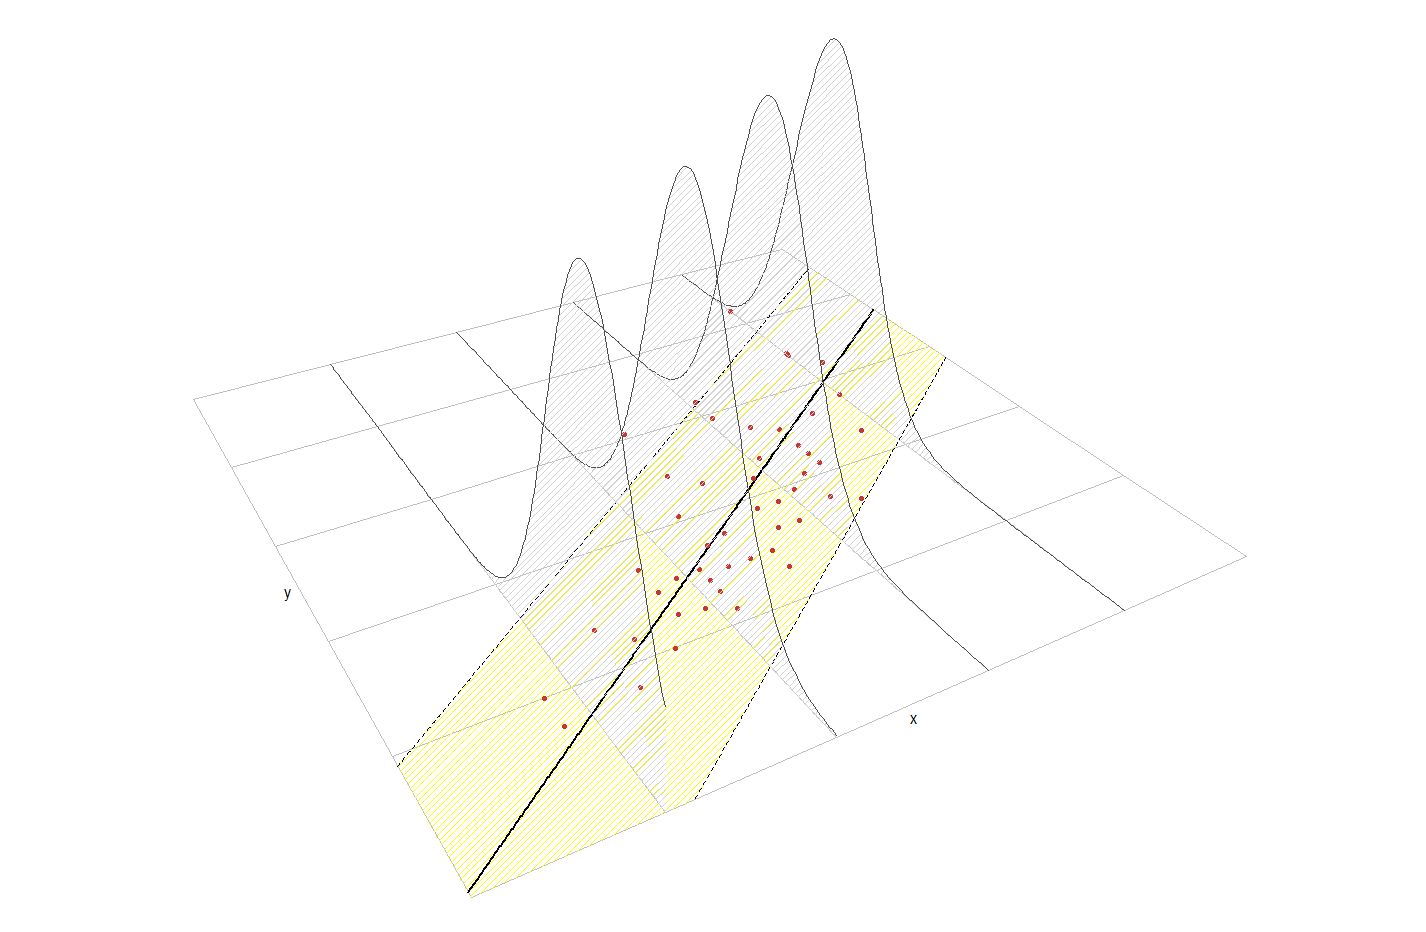
\includegraphics[width=0.9\linewidth]{images/figures/RegresiaLiniara} 

}

\caption{Regresia liniara simpla}\label{fig:unnamed-chunk-3}
\end{figure}

Dat fiind un eșantion \((X_1,Y_1),\ldots,(X_n,Y_n)\) pentru variabilele
\(X\) și \(Y\) putem estima coeficienții necunoscuți \(\beta_0\) și
\(\beta_1\) minimizând \emph{suma abaterilor pătratice reziduale}
(\emph{Residual Sum of Squares} - RSS)

\[
\text{RSS}(\beta_0,\beta_1)=\sum_{i=1}^n(Y_i-\beta_0-\beta_1X_i)^2
\]

ceea ce conduce la

\[
\hat\beta_0=\bar{Y}-\hat\beta_1\bar{X},\quad \hat\beta_1=\frac{s_{xy}}{s_x^2}=\frac{\sum_{i=1}^{n}{(X_i-\bar{X})}Y_i}{\sum_{i=1}^{n}{(X_i-\bar{X})^2}}
\]

unde

\begin{itemize}
\tightlist
\item
  \(\bar{X}=\frac{1}{n}\sum_{i=1}^nX_i\) este \emph{media eșantionului}
\item
  \(s_x^2=\frac{1}{n}\sum_{i=1}^n(X_i-\bar{X})^2\) este \emph{varianța
  eșantionului}
\item
  \(s_{xy}=\frac{1}{n}\sum_{i=1}^n(X_i-\bar{X})(Y_i-\bar{Y})\) este
  \emph{covarianța eșantionului}
\end{itemize}

\begin{figure}

{\centering 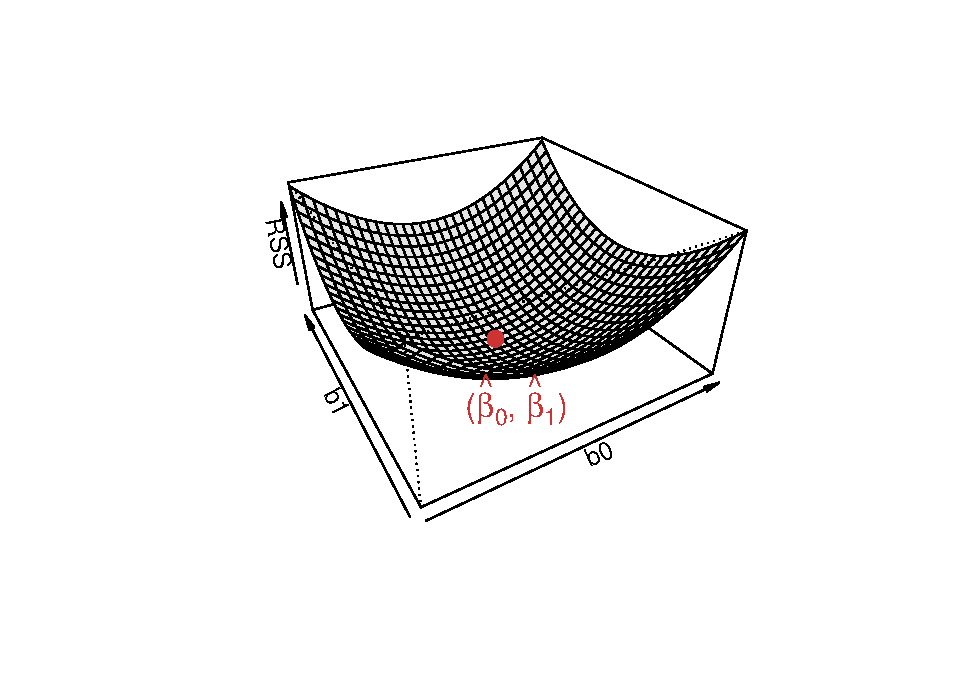
\includegraphics[width=0.9\linewidth]{Lab_7_8_files/figure-latex/unnamed-chunk-4-1} 

}

\caption{Graficul functiei RSS pentru modelul $y = -0.5 + 1.5x + e$.}\label{fig:unnamed-chunk-4}
\end{figure}

Odată ce avem estimatorii \((\hat\beta_0,\hat\beta_1)\) , putem defini:

\begin{itemize}
\tightlist
\item
  \emph{valorile prognozate} (\emph{fitted values})
  \(\hat Y_1,\ldots,\hat Y_n\) (valorile verticale pe dreapta de
  regresie), unde
\end{itemize}

\[
\hat Y_i=\hat\beta_0+\hat\beta_1X_i,\quad i=1,\ldots,n
\]

\begin{itemize}
\tightlist
\item
  \emph{reziduurile estimate} (\emph{estimated residuals})
  \(\hat \varepsilon_1,\ldots,\hat \varepsilon_n\) (distanțele verticale
  dintre punctele actuale \((X_i,Y_i)\) și cele prognozate
  \((X_i,\hat Y_i)\)), unde
\end{itemize}

\[
\hat\varepsilon_i=Y_i-\hat Y_i,\quad i=1,\ldots,n
\]

Estimatorul pentru \(\sigma^2\) este \[
\hat{\sigma}^2 = \frac{RSS(\hat{\beta}_0,\hat{\beta}_1)}{n-2} = \frac{\sum_{i=1}^{n}\hat{\varepsilon}_i^2}{n-2}.
\]

\subsection{Exemplul 1}\label{exemplul-1}

\begin{quote}
În acest exercițiu vrem să investigăm relația dintre consumul de clorură
de sodiu (sarea de bucătărie) și tensiunea arterială la persoanele
trecute de 65 de ani. Pentru aceasta vom folosi setul de date
\href{data/saltBP.txt}{\texttt{saltBP}} care conține informații despre
tensiunea arterială a 25 de pacienți.
\end{quote}

Începem prin a înregistra setul de date

\begin{Shaded}
\begin{Highlighting}[]
\NormalTok{saltBP =}\StringTok{ }\KeywordTok{read.table}\NormalTok{(}\StringTok{"data/saltBP.txt"}\NormalTok{, }\DataTypeTok{header =} \NormalTok{T)}

\KeywordTok{plot}\NormalTok{(saltBP$salt, saltBP$BP, }
     \DataTypeTok{xlab =} \StringTok{"sare"}\NormalTok{, }
     \DataTypeTok{ylab =} \StringTok{"tensiunea arteriala"}\NormalTok{, }
     \DataTypeTok{col =} \StringTok{"brown3"}\NormalTok{, }
     \DataTypeTok{pch =} \DecValTok{16}\NormalTok{, }
     \DataTypeTok{bty=}\StringTok{"n"}\NormalTok{)}
\end{Highlighting}
\end{Shaded}

\begin{figure}

{\centering 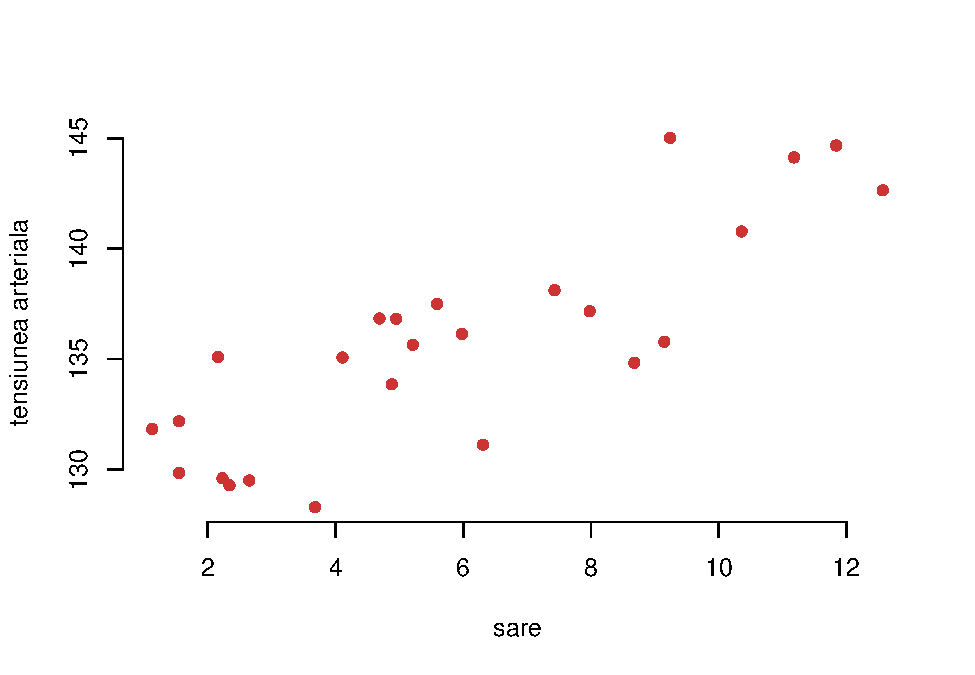
\includegraphics[width=0.9\linewidth]{Lab_7_8_files/figure-latex/unnamed-chunk-5-1} 

}

\caption{Diagrama de imprastiere}\label{fig:unnamed-chunk-5}
\end{figure}

\begin{Shaded}
\begin{Highlighting}[]
\KeywordTok{summary}\NormalTok{(saltBP)}
\end{Highlighting}
\end{Shaded}

\begin{verbatim}
##        BP             salt          saltLevel  
##  Min.   :128.3   Min.   : 1.130   Min.   :0.0  
##  1st Qu.:131.8   1st Qu.: 2.650   1st Qu.:0.0  
##  Median :135.7   Median : 5.210   Median :0.0  
##  Mean   :135.7   Mean   : 5.898   Mean   :0.4  
##  3rd Qu.:137.5   3rd Qu.: 8.680   3rd Qu.:1.0  
##  Max.   :145.0   Max.   :12.570   Max.   :1.0
\end{verbatim}

\subsubsection{Estimarea parametrilor}\label{estimarea-parametrilor}

Considerăm modelul de regresie \(Y = \beta_0 + \beta_1 X + \varepsilon\)
(unde \(X=\)\texttt{saltBP\$salt} iar \(Y=\)\texttt{saltBP\$BP}),
\(\varepsilon\sim \mathcal{N}(0,\sigma^2)\), a cărui parametrii sunt
\(\beta_0\), \(\beta_1\) și \(\sigma^2\).

\begin{itemize}
\tightlist
\item
  estimatorii parametrilor \(\beta_0\) și \(\beta_1\)
\end{itemize}

\begin{Shaded}
\begin{Highlighting}[]
\CommentTok{# pentru b1}

\NormalTok{b1 =}\StringTok{ }\KeywordTok{cov}\NormalTok{(saltBP$salt, saltBP$BP)/}\KeywordTok{var}\NormalTok{(saltBP$salt)}
\KeywordTok{cat}\NormalTok{(}\StringTok{"b1 = "}\NormalTok{, b1)}
\end{Highlighting}
\end{Shaded}

\begin{verbatim}
## b1 =  1.196894
\end{verbatim}

\begin{Shaded}
\begin{Highlighting}[]
\CommentTok{# sau }

\KeywordTok{sum}\NormalTok{((saltBP$salt-}\KeywordTok{mean}\NormalTok{(saltBP$salt))*(saltBP$BP))/}\KeywordTok{sum}\NormalTok{((saltBP$salt-}\KeywordTok{mean}\NormalTok{(saltBP$salt))^}\DecValTok{2}\NormalTok{)}
\end{Highlighting}
\end{Shaded}

\begin{verbatim}
## [1] 1.196894
\end{verbatim}

\begin{Shaded}
\begin{Highlighting}[]
\CommentTok{# pentru b0}

\NormalTok{b0 =}\StringTok{ }\KeywordTok{mean}\NormalTok{(saltBP$BP) -}\StringTok{ }\NormalTok{b1*}\KeywordTok{mean}\NormalTok{(saltBP$salt)}
\KeywordTok{cat}\NormalTok{(}\StringTok{"b0 = "}\NormalTok{, b0)}
\end{Highlighting}
\end{Shaded}

\begin{verbatim}
## b0 =  128.6164
\end{verbatim}

sau folosind funcția \texttt{lm}:

\begin{Shaded}
\begin{Highlighting}[]
\NormalTok{saltBP_model =}\StringTok{ }\KeywordTok{lm}\NormalTok{(BP~salt, }\DataTypeTok{data =} \NormalTok{saltBP)}
\KeywordTok{names}\NormalTok{(saltBP_model)}
\end{Highlighting}
\end{Shaded}

\begin{verbatim}
##  [1] "coefficients"  "residuals"     "effects"       "rank"         
##  [5] "fitted.values" "assign"        "qr"            "df.residual"  
##  [9] "xlevels"       "call"          "terms"         "model"
\end{verbatim}

\begin{Shaded}
\begin{Highlighting}[]
\NormalTok{saltBP_model$coefficients}
\end{Highlighting}
\end{Shaded}

\begin{verbatim}
## (Intercept)        salt 
##  128.616397    1.196894
\end{verbatim}

Dreapta de regresie este:

\begin{Shaded}
\begin{Highlighting}[]
\KeywordTok{plot}\NormalTok{(saltBP$salt, saltBP$BP, }
     \DataTypeTok{xlab =} \StringTok{"nivelul de sare"}\NormalTok{, }
     \DataTypeTok{ylab =} \StringTok{"tensiunea arteriala"}\NormalTok{, }
     \DataTypeTok{col =} \StringTok{"brown3"}\NormalTok{, }
     \DataTypeTok{pch =} \DecValTok{16}\NormalTok{, }
     \DataTypeTok{bty=}\StringTok{"n"}\NormalTok{, }
     \DataTypeTok{main =} \KeywordTok{paste}\NormalTok{(}\StringTok{"y = "}\NormalTok{, }\KeywordTok{format}\NormalTok{(b0, }\DataTypeTok{digits =} \DecValTok{4}\NormalTok{), }\StringTok{" + "}\NormalTok{, }\KeywordTok{format}\NormalTok{(b1, }\DataTypeTok{digits =} \DecValTok{4}\NormalTok{), }\StringTok{" x"}\NormalTok{))}

\KeywordTok{abline}\NormalTok{(}\DataTypeTok{a =} \NormalTok{b0, }\DataTypeTok{b =} \NormalTok{b1, }\DataTypeTok{col =} \StringTok{"grey"}\NormalTok{, }\DataTypeTok{lwd =} \DecValTok{2}\NormalTok{)}
\KeywordTok{points}\NormalTok{(}\KeywordTok{mean}\NormalTok{(saltBP$salt), }\KeywordTok{mean}\NormalTok{(saltBP$BP), }\DataTypeTok{pch =} \DecValTok{16}\NormalTok{, }\DataTypeTok{col =} \StringTok{"dark green"}\NormalTok{, }\DataTypeTok{cex =} \FloatTok{1.2}\NormalTok{)}
\KeywordTok{text}\NormalTok{(}\KeywordTok{mean}\NormalTok{(saltBP$salt), }\KeywordTok{mean}\NormalTok{(saltBP$BP)-}\FloatTok{1.3}\NormalTok{, }\DataTypeTok{col =} \StringTok{"dark green"}\NormalTok{, }\DataTypeTok{cex =} \FloatTok{1.2}\NormalTok{, }
     \DataTypeTok{labels =} \KeywordTok{expression}\NormalTok{(}\KeywordTok{paste}\NormalTok{(}\StringTok{"("}\NormalTok{, }\KeywordTok{bar}\NormalTok{(x), }\StringTok{","}\NormalTok{, }\KeywordTok{bar}\NormalTok{(y),}\StringTok{")"}\NormalTok{)))}
\end{Highlighting}
\end{Shaded}

\begin{figure}

{\centering 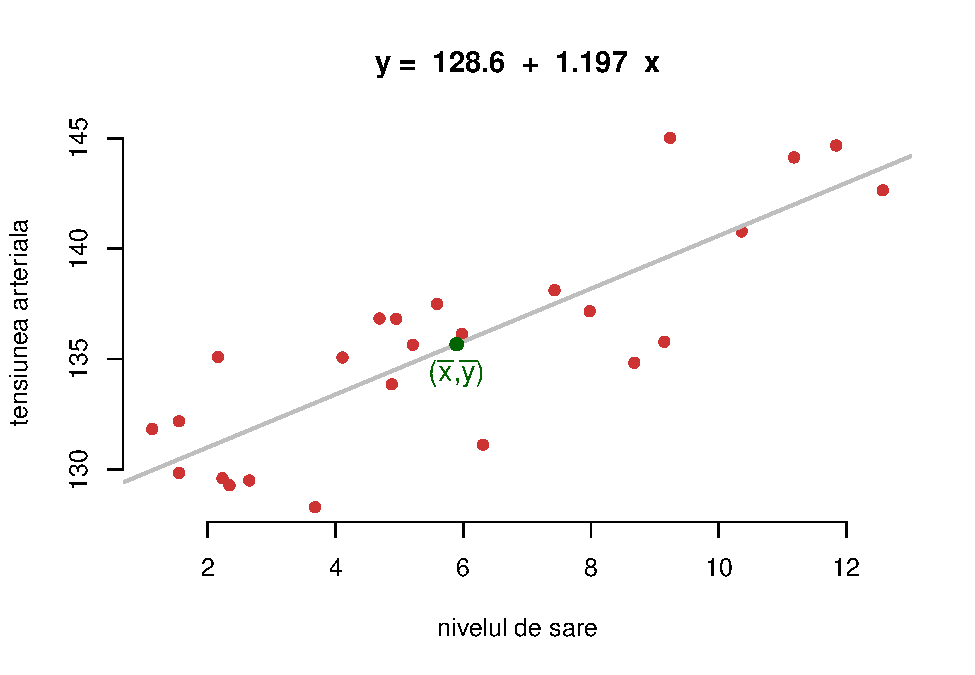
\includegraphics[width=0.9\linewidth]{Lab_7_8_files/figure-latex/unnamed-chunk-10-1} 

}

\caption{Dreapta de regresie}\label{fig:unnamed-chunk-10}
\end{figure}

\begin{itemize}
\tightlist
\item
  estimatorul lui \(\sigma\) (\(\hat{\sigma}\))
\end{itemize}

\begin{Shaded}
\begin{Highlighting}[]
\NormalTok{n =}\StringTok{ }\KeywordTok{length}\NormalTok{(saltBP$BP)}
\NormalTok{e_hat =}\StringTok{ }\NormalTok{saltBP$BP -}\StringTok{ }\NormalTok{(b0+b1*saltBP$salt)}

\NormalTok{rss =}\StringTok{ }\KeywordTok{sum}\NormalTok{(e_hat^}\DecValTok{2}\NormalTok{)}

\NormalTok{sigma_hat =}\StringTok{ }\KeywordTok{sqrt}\NormalTok{(rss/(n}\DecValTok{-2}\NormalTok{))}
\NormalTok{sigma_hat}
\end{Highlighting}
\end{Shaded}

\begin{verbatim}
## [1] 2.745374
\end{verbatim}

sau cu ajutorul funcției \texttt{lm}

\begin{Shaded}
\begin{Highlighting}[]
\KeywordTok{sqrt}\NormalTok{(}\KeywordTok{deviance}\NormalTok{(saltBP_model)/}\KeywordTok{df.residual}\NormalTok{(saltBP_model))}
\end{Highlighting}
\end{Shaded}

\begin{verbatim}
## [1] 2.745374
\end{verbatim}

sau încă

\begin{Shaded}
\begin{Highlighting}[]
\NormalTok{saltBP_model_summary =}\StringTok{ }\KeywordTok{summary}\NormalTok{(saltBP_model)}
\CommentTok{# names(saltBP_model_summary)}
\NormalTok{saltBP_model_summary$sigma}
\end{Highlighting}
\end{Shaded}

\begin{verbatim}
## [1] 2.745374
\end{verbatim}

\subsubsection{Intervale de încredere pentru
parametrii}\label{intervale-de-incredere-pentru-parametrii}

Repartițiile lui \(\hat\beta_0\) și \(\hat\beta_1\) sunt

\[
\hat\beta_0\sim\mathcal{N}\left(\beta_0,\mathrm{SE}(\hat\beta_0)^2\right),\quad\hat\beta_1\sim\mathcal{N}\left(\beta_1,\mathrm{SE}(\hat\beta_1)^2\right)
\]

unde

\[
\mathrm{SE}(\hat\beta_0)^2=\frac{\sigma^2}{n}\left[1+\frac{\bar X^2}{s_x^2}\right],\quad \mathrm{SE}(\hat\beta_1)^2=\frac{\sigma^2}{ns_x^2}.
\]

Folosind estimatorul \(\hat\sigma^2\) pentru \(\sigma^2\) obținem că

\[
\frac{\hat\beta_0-\beta_0}{\hat{\mathrm{SE}}(\hat\beta_0)}\sim t_{n-2},\quad\frac{\hat\beta_1-\beta_1}{\hat{\mathrm{SE}}(\hat\beta_1)}\sim t_{n-2}
\]

unde

\[
\hat{\mathrm{SE}}(\hat\beta_0)^2=\frac{\hat\sigma^2}{n}\left[1+\frac{\bar X^2}{s_x^2}\right],\quad \hat{\mathrm{SE}}(\hat\beta_1)^2=\frac{\hat\sigma^2}{ns_x^2}
\]

prin urmare, intervalele de încredere de nivel \(1-\alpha\) pentru
\(\beta_0\) și \(\beta_1\) sunt

\[
IC = \left(\hat\beta_j\pm\hat{\mathrm{SE}}(\hat\beta_j)t_{n-2;\alpha/2}\right),\quad j=0,1.
\]

\begin{Shaded}
\begin{Highlighting}[]
\NormalTok{alpha =}\StringTok{ }\FloatTok{0.05}

\CommentTok{# trebuie avut grija ca functia var si sd calculeaza impartind la (n-1) si nu la n !!!}
\NormalTok{se_b0 =}\StringTok{ }\KeywordTok{sqrt}\NormalTok{(sigma_hat^}\DecValTok{2}\NormalTok{*(}\DecValTok{1}\NormalTok{/n+}\KeywordTok{mean}\NormalTok{(saltBP$salt)^}\DecValTok{2}\NormalTok{/((n}\DecValTok{-1}\NormalTok{)*}\KeywordTok{var}\NormalTok{(saltBP$salt))))}
\NormalTok{se_b1 =}\StringTok{ }\KeywordTok{sqrt}\NormalTok{(sigma_hat^}\DecValTok{2}\NormalTok{/((n}\DecValTok{-1}\NormalTok{)*}\KeywordTok{var}\NormalTok{(saltBP$salt)))}

\NormalTok{lw_b0 =}\StringTok{ }\NormalTok{b0 -}\StringTok{ }\KeywordTok{qt}\NormalTok{(}\DecValTok{1}\NormalTok{-alpha/}\DecValTok{2}\NormalTok{, n}\DecValTok{-2}\NormalTok{)*se_b0}
\NormalTok{up_b0 =}\StringTok{ }\NormalTok{b0 +}\StringTok{ }\KeywordTok{qt}\NormalTok{(}\DecValTok{1}\NormalTok{-alpha/}\DecValTok{2}\NormalTok{, n}\DecValTok{-2}\NormalTok{)*se_b0}

\KeywordTok{cat}\NormalTok{(}\StringTok{"CI pentru b0 este ("}\NormalTok{, lw_b0, }\StringTok{", "}\NormalTok{, up_b0, }\StringTok{")}\CharTok{\textbackslash{}n}\StringTok{"}\NormalTok{)}
\end{Highlighting}
\end{Shaded}

\begin{verbatim}
## CI pentru b0 este ( 126.337 ,  130.8958 )
\end{verbatim}

\begin{Shaded}
\begin{Highlighting}[]
\NormalTok{lw_b1 =}\StringTok{ }\NormalTok{b1 -}\StringTok{ }\KeywordTok{qt}\NormalTok{(}\DecValTok{1}\NormalTok{-alpha/}\DecValTok{2}\NormalTok{, n}\DecValTok{-2}\NormalTok{)*se_b1}
\NormalTok{up_b1 =}\StringTok{ }\NormalTok{b1 +}\StringTok{ }\KeywordTok{qt}\NormalTok{(}\DecValTok{1}\NormalTok{-alpha/}\DecValTok{2}\NormalTok{, n}\DecValTok{-2}\NormalTok{)*se_b1}
  
\KeywordTok{cat}\NormalTok{(}\StringTok{"CI pentru b1 este ("}\NormalTok{, lw_b1, }\StringTok{", "}\NormalTok{, up_b1, }\StringTok{")"}\NormalTok{)}
\end{Highlighting}
\end{Shaded}

\begin{verbatim}
## CI pentru b1 este ( 0.8617951 ,  1.531993 )
\end{verbatim}

Același rezultat se obține apelând funcția \texttt{confint} :

\begin{Shaded}
\begin{Highlighting}[]
\KeywordTok{confint}\NormalTok{(saltBP_model)}
\end{Highlighting}
\end{Shaded}

\begin{verbatim}
##                   2.5 %     97.5 %
## (Intercept) 126.3369606 130.895834
## salt          0.8617951   1.531993
\end{verbatim}

Putem construi și o regiune de încredere pentru perechea
\((\beta_0, \beta_1)\):

\begin{Shaded}
\begin{Highlighting}[]
\KeywordTok{plot}\NormalTok{(}\KeywordTok{ellipse}\NormalTok{(saltBP_model, }\KeywordTok{c}\NormalTok{(}\DecValTok{1}\NormalTok{,}\DecValTok{2}\NormalTok{)), }\DataTypeTok{type =} \StringTok{"l"}\NormalTok{, }\DataTypeTok{col =} \StringTok{"grey30"}\NormalTok{, }
     \DataTypeTok{xlab =} \KeywordTok{expression}\NormalTok{(beta[}\DecValTok{0}\NormalTok{]), }
     \DataTypeTok{ylab =} \KeywordTok{expression}\NormalTok{(beta[}\DecValTok{1}\NormalTok{]), }
     \DataTypeTok{bty =} \StringTok{"n"}\NormalTok{)}
\KeywordTok{points}\NormalTok{(}\KeywordTok{coef}\NormalTok{(saltBP_model)[}\DecValTok{1}\NormalTok{], }\KeywordTok{coef}\NormalTok{(saltBP_model)[}\DecValTok{2}\NormalTok{], }\DataTypeTok{pch =} \DecValTok{18}\NormalTok{, }\DataTypeTok{col =} \StringTok{"brown3"}\NormalTok{)}
\KeywordTok{abline}\NormalTok{(}\DataTypeTok{v =} \KeywordTok{confint}\NormalTok{(saltBP_model)[}\DecValTok{1}\NormalTok{,], }\DataTypeTok{lty =} \DecValTok{2}\NormalTok{)}
\KeywordTok{abline}\NormalTok{(}\DataTypeTok{h =} \KeywordTok{confint}\NormalTok{(saltBP_model)[}\DecValTok{2}\NormalTok{,], }\DataTypeTok{lty =} \DecValTok{2}\NormalTok{)}
\end{Highlighting}
\end{Shaded}

\begin{figure}

{\centering 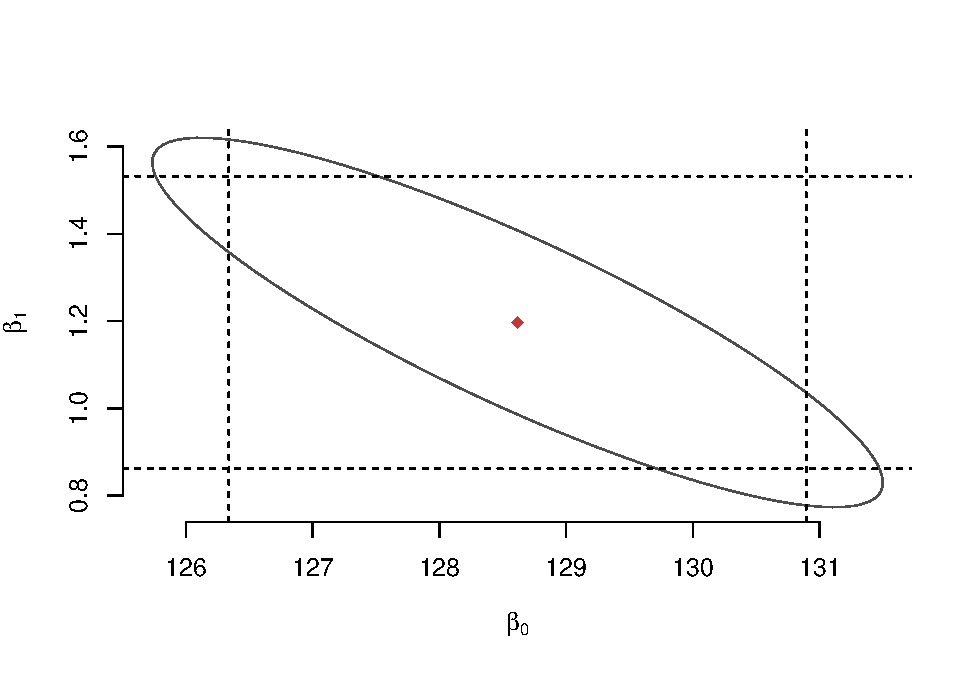
\includegraphics[width=0.9\linewidth]{Lab_7_8_files/figure-latex/unnamed-chunk-16-1} 

}

\caption{Regiune de incredere}\label{fig:unnamed-chunk-16}
\end{figure}

\subsubsection{ANOVA pentru regresie}\label{anova-pentru-regresie}

Este predictorul \(X\) folositor în prezicerea răspunsului \(Y\) ? Vrem
să testăm ipoteza nulă \(H_0:\;\beta_1=0\).

Introducem următoarele \emph{sume de abateri pătratice}:

\begin{itemize}
\tightlist
\item
  \(SS_T=\sum_{i=1}^n\left(Y_i-\bar Y\right)^2\), \textbf{suma
  abaterilor pătratice totală} (variația totală a lui
  \(Y_1,\ldots,Y_n\)).
\item
  \(SS_{reg}=\sum_{i=1}^n\left(\hat Y_i-\bar Y\right)^2\), \textbf{suma
  abaterilor pătratice de regresie} (variabilitatea explicată de dreapta
  de regresie)
\item
  \(RSS=\sum_{i=1}^n\left(Y_i-\hat Y_i\right)^2\), \textbf{suma
  abaterilor pătratice reziduale}
\end{itemize}

Avem următoarea descompunere ANOVA

\[
\underbrace{SS_T}_{\text{Variația lui }Y_i} = \underbrace{SS_{reg}}_{\text{Variația lui }\hat Y_i} + \underbrace{RSS}_{\text{Variația lui }\hat \varepsilon_i} 
\]

și tabelul ANOVA corespunzător

\begin{longtable}[]{@{}llllll@{}}
\toprule
& Df & SS & MS & \(F\) & \(p\)-value\tabularnewline
\midrule
\endhead
Predictor & \(1\) & \(SS_{reg}\) & \(\frac{SS_{reg}}{1}\) &
\(\frac{SS_{reg}/1}{RSS/(n-2)}\) & \(p\)\tabularnewline
Residuuri & \(n - 2\) & \(RSS\) & \(\frac{RSS}{n-2}\) & &\tabularnewline
\bottomrule
\end{longtable}

Descompunerea ANOVA pentru problema noastră poate fi ilustrată astfel:

\begin{itemize}
\tightlist
\item
  \emph{suma abaterilor pătratice totală}:
\end{itemize}

\begin{Shaded}
\begin{Highlighting}[]
\KeywordTok{plot}\NormalTok{(saltBP$salt, saltBP$BP, }\DataTypeTok{pch =} \DecValTok{16}\NormalTok{, }\DataTypeTok{type =} \StringTok{"n"}\NormalTok{,}
     \DataTypeTok{main =} \KeywordTok{paste}\NormalTok{(}\StringTok{"SST ="}\NormalTok{, }\KeywordTok{round}\NormalTok{(}\KeywordTok{sum}\NormalTok{((saltBP$BP -}\StringTok{ }\KeywordTok{mean}\NormalTok{(saltBP$BP))^}\DecValTok{2}\NormalTok{), }\DecValTok{2}\NormalTok{)), }
     \DataTypeTok{col.main =} \StringTok{"brown4"}\NormalTok{, }
     \DataTypeTok{xlab =} \StringTok{"nivelul de sare"}\NormalTok{, }
     \DataTypeTok{ylab =} \StringTok{"tensiunea arteriala"}\NormalTok{, }
     \DataTypeTok{bty =} \StringTok{"n"}\NormalTok{)}

\KeywordTok{abline}\NormalTok{(saltBP_model$coefficients, }\DataTypeTok{col =} \StringTok{"grey30"}\NormalTok{, }\DataTypeTok{lwd =} \DecValTok{2}\NormalTok{)}
\KeywordTok{abline}\NormalTok{(}\DataTypeTok{h =} \KeywordTok{mean}\NormalTok{(saltBP$BP), }\DataTypeTok{col =} \StringTok{"brown2"}\NormalTok{, }\DataTypeTok{lty =} \DecValTok{2}\NormalTok{)}

\KeywordTok{segments}\NormalTok{(}\DataTypeTok{x0 =} \NormalTok{saltBP$salt, }\DataTypeTok{y0 =} \KeywordTok{mean}\NormalTok{(saltBP$BP), }
         \DataTypeTok{x1 =} \NormalTok{saltBP$salt, }\DataTypeTok{y1 =} \NormalTok{saltBP$BP, }
         \DataTypeTok{col =} \StringTok{"grey50"}\NormalTok{, }\DataTypeTok{lwd =} \DecValTok{2}\NormalTok{, }\DataTypeTok{lty =} \DecValTok{2}\NormalTok{)}

\KeywordTok{legend}\NormalTok{(}\StringTok{"topleft"}\NormalTok{, }
       \DataTypeTok{legend =} \KeywordTok{expression}\NormalTok{(}\StringTok{"Dreapta de regresie"}\NormalTok{, }\StringTok{"Media esantionului "} \NormalTok{*}\StringTok{ }\KeywordTok{bar}\NormalTok{(Y),}
                                      \NormalTok{(Y[i] -}\StringTok{ }\KeywordTok{bar}\NormalTok{(Y))^}\DecValTok{2}\NormalTok{), }
       \DataTypeTok{lwd =} \KeywordTok{c}\NormalTok{(}\DecValTok{2}\NormalTok{, }\DecValTok{1}\NormalTok{, }\DecValTok{2}\NormalTok{),}
       \DataTypeTok{col =} \KeywordTok{c}\NormalTok{(}\StringTok{"grey30"}\NormalTok{, }\StringTok{"brown2"}\NormalTok{, }\StringTok{"grey50"}\NormalTok{), }
       \DataTypeTok{lty =} \KeywordTok{c}\NormalTok{(}\DecValTok{1}\NormalTok{, }\DecValTok{2}\NormalTok{, }\DecValTok{2}\NormalTok{), }
       \DataTypeTok{bty =} \StringTok{"n"}\NormalTok{)}

\KeywordTok{points}\NormalTok{(saltBP$salt, saltBP$BP, }\DataTypeTok{pch =} \DecValTok{16}\NormalTok{, }\DataTypeTok{col =} \StringTok{"brown3"}\NormalTok{)}
\end{Highlighting}
\end{Shaded}

\begin{center}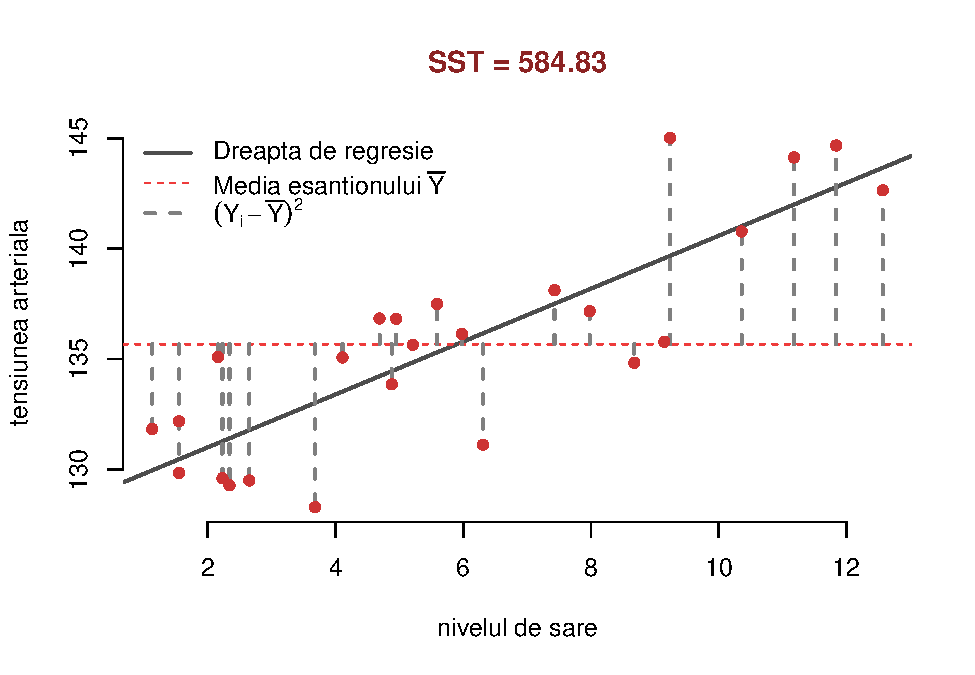
\includegraphics[width=0.9\linewidth]{Lab_7_8_files/figure-latex/unnamed-chunk-17-1} \end{center}

\begin{itemize}
\tightlist
\item
  \emph{suma abaterilor pătratice de regresie}
\end{itemize}

\begin{Shaded}
\begin{Highlighting}[]
\KeywordTok{plot}\NormalTok{(saltBP$salt, saltBP$BP, }\DataTypeTok{pch =} \DecValTok{16}\NormalTok{, }\DataTypeTok{type =} \StringTok{"n"}\NormalTok{,}
     \DataTypeTok{main =} \KeywordTok{paste}\NormalTok{(}\StringTok{"SSreg ="}\NormalTok{, }
                  \KeywordTok{round}\NormalTok{(}\KeywordTok{sum}\NormalTok{((saltBP_model$fitted.values -}\StringTok{ }\KeywordTok{mean}\NormalTok{(saltBP$BP))^}\DecValTok{2}\NormalTok{), }\DecValTok{2}\NormalTok{)), }
     \DataTypeTok{col.main =} \StringTok{"forestgreen"}\NormalTok{, }
     \DataTypeTok{xlab =} \StringTok{"nivelul de sare"}\NormalTok{, }
     \DataTypeTok{ylab =} \StringTok{"tensiunea arteriala"}\NormalTok{, }
     \DataTypeTok{bty =} \StringTok{"n"}\NormalTok{)}

\KeywordTok{abline}\NormalTok{(saltBP_model$coefficients, }\DataTypeTok{col =} \StringTok{"grey30"}\NormalTok{, }\DataTypeTok{lwd =} \DecValTok{2}\NormalTok{)}
\KeywordTok{abline}\NormalTok{(}\DataTypeTok{h =} \KeywordTok{mean}\NormalTok{(saltBP$BP), }\DataTypeTok{col =} \StringTok{"brown2"}\NormalTok{, }\DataTypeTok{lty =} \DecValTok{2}\NormalTok{)}

\KeywordTok{segments}\NormalTok{(}\DataTypeTok{x0 =} \NormalTok{saltBP$salt, }\DataTypeTok{y0 =} \KeywordTok{mean}\NormalTok{(saltBP$BP), }
         \DataTypeTok{x1 =} \NormalTok{saltBP$salt, }\DataTypeTok{y1 =} \NormalTok{saltBP_model$fitted.values, }
         \DataTypeTok{col =} \StringTok{"forestgreen"}\NormalTok{, }\DataTypeTok{lwd =} \DecValTok{2}\NormalTok{, }\DataTypeTok{lty =} \DecValTok{2}\NormalTok{)}

\KeywordTok{points}\NormalTok{(saltBP$salt, saltBP_model$fitted.values, }\DataTypeTok{pch =} \DecValTok{16}\NormalTok{, }\DataTypeTok{col =} \StringTok{"forestgreen"}\NormalTok{)}

\KeywordTok{legend}\NormalTok{(}\StringTok{"topleft"}\NormalTok{, }
       \DataTypeTok{legend =} \KeywordTok{expression}\NormalTok{(}\StringTok{"Dreapta de regresie"}\NormalTok{, }\StringTok{"Media esantionului "} \NormalTok{*}\StringTok{ }\KeywordTok{bar}\NormalTok{(Y),}
                                      \NormalTok{(}\KeywordTok{hat}\NormalTok{(Y)[i] -}\StringTok{ }\KeywordTok{bar}\NormalTok{(Y))^}\DecValTok{2}\NormalTok{), }
       \DataTypeTok{lwd =} \KeywordTok{c}\NormalTok{(}\DecValTok{2}\NormalTok{, }\DecValTok{1}\NormalTok{, }\DecValTok{2}\NormalTok{),}
       \DataTypeTok{col =} \KeywordTok{c}\NormalTok{(}\StringTok{"grey30"}\NormalTok{, }\StringTok{"brown2"}\NormalTok{, }\StringTok{"forestgreen"}\NormalTok{), }
       \DataTypeTok{lty =} \KeywordTok{c}\NormalTok{(}\DecValTok{1}\NormalTok{, }\DecValTok{2}\NormalTok{, }\DecValTok{2}\NormalTok{), }
       \DataTypeTok{bty =} \StringTok{"n"}\NormalTok{)}

\KeywordTok{points}\NormalTok{(saltBP$salt, saltBP$BP, }\DataTypeTok{pch =} \DecValTok{16}\NormalTok{, }\DataTypeTok{col =} \StringTok{"brown3"}\NormalTok{)}
\end{Highlighting}
\end{Shaded}

\begin{center}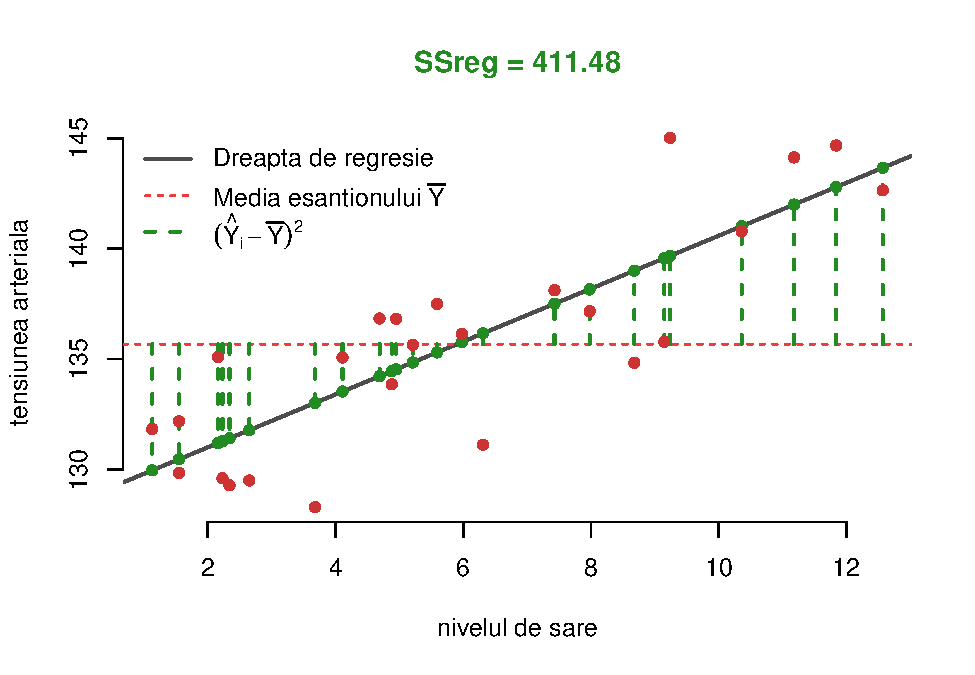
\includegraphics[width=0.9\linewidth]{Lab_7_8_files/figure-latex/unnamed-chunk-18-1} \end{center}

\begin{itemize}
\tightlist
\item
  \emph{suma abaterilor pătratice reziduale}
\end{itemize}

\begin{Shaded}
\begin{Highlighting}[]
\KeywordTok{plot}\NormalTok{(saltBP$salt, saltBP$BP, }\DataTypeTok{pch =} \DecValTok{16}\NormalTok{, }\DataTypeTok{type =} \StringTok{"n"}\NormalTok{,}
     \DataTypeTok{main =} \KeywordTok{paste}\NormalTok{(}\StringTok{"RSS ="}\NormalTok{, }
                  \KeywordTok{round}\NormalTok{(}\KeywordTok{sum}\NormalTok{((saltBP$BP -}\StringTok{ }\NormalTok{saltBP_model$fitted.values)^}\DecValTok{2}\NormalTok{), }\DecValTok{2}\NormalTok{)), }
     \DataTypeTok{col.main =} \StringTok{"orange"}\NormalTok{, }
     \DataTypeTok{xlab =} \StringTok{"nivelul de sare"}\NormalTok{, }
     \DataTypeTok{ylab =} \StringTok{"tensiunea arteriala"}\NormalTok{, }
     \DataTypeTok{bty =} \StringTok{"n"}\NormalTok{)}

\KeywordTok{abline}\NormalTok{(saltBP_model$coefficients, }\DataTypeTok{col =} \StringTok{"grey30"}\NormalTok{, }\DataTypeTok{lwd =} \DecValTok{2}\NormalTok{)}

\KeywordTok{segments}\NormalTok{(}\DataTypeTok{x0 =} \NormalTok{saltBP$salt, }\DataTypeTok{y0 =} \NormalTok{saltBP$BP, }
         \DataTypeTok{x1 =} \NormalTok{saltBP$salt, }\DataTypeTok{y1 =} \NormalTok{saltBP_model$fitted.values, }
         \DataTypeTok{col =} \StringTok{"orange"}\NormalTok{, }\DataTypeTok{lwd =} \DecValTok{2}\NormalTok{, }\DataTypeTok{lty =} \DecValTok{2}\NormalTok{)}

\KeywordTok{points}\NormalTok{(saltBP$salt, saltBP_model$fitted.values, }\DataTypeTok{pch =} \DecValTok{16}\NormalTok{, }\DataTypeTok{col =} \StringTok{"orange"}\NormalTok{)}

\KeywordTok{legend}\NormalTok{(}\StringTok{"topleft"}\NormalTok{, }
       \DataTypeTok{legend =} \KeywordTok{expression}\NormalTok{(}\StringTok{"Dreapta de regresie"}\NormalTok{, (}\KeywordTok{hat}\NormalTok{(Y)[i] -}\StringTok{ }\NormalTok{Y[i])^}\DecValTok{2}\NormalTok{), }
       \DataTypeTok{lwd =} \KeywordTok{c}\NormalTok{(}\DecValTok{2}\NormalTok{, }\DecValTok{2}\NormalTok{),}
       \DataTypeTok{col =} \KeywordTok{c}\NormalTok{(}\StringTok{"grey30"}\NormalTok{, }\StringTok{"orange"}\NormalTok{), }
       \DataTypeTok{lty =} \KeywordTok{c}\NormalTok{(}\DecValTok{1}\NormalTok{, }\DecValTok{2}\NormalTok{), }
       \DataTypeTok{bty =} \StringTok{"n"}\NormalTok{)}

\KeywordTok{points}\NormalTok{(saltBP$salt, saltBP$BP, }\DataTypeTok{pch =} \DecValTok{16}\NormalTok{, }\DataTypeTok{col =} \StringTok{"brown3"}\NormalTok{)}
\end{Highlighting}
\end{Shaded}

\begin{center}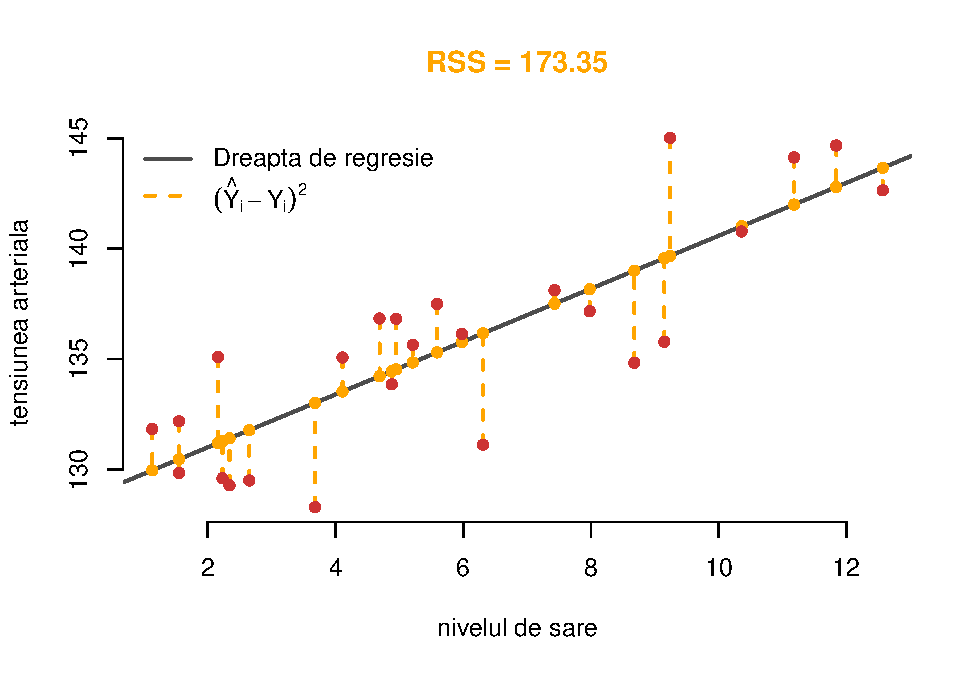
\includegraphics[width=0.9\linewidth]{Lab_7_8_files/figure-latex/unnamed-chunk-19-1} \end{center}

Tabelul ANOVA se obține prin

\begin{Shaded}
\begin{Highlighting}[]
\CommentTok{# tabel ANOVA }
\KeywordTok{anova}\NormalTok{(saltBP_model)}
\end{Highlighting}
\end{Shaded}

\begin{verbatim}
## Analysis of Variance Table
## 
## Response: BP
##           Df Sum Sq Mean Sq F value    Pr(>F)    
## salt       1 411.48  411.48  54.594 1.631e-07 ***
## Residuals 23 173.35    7.54                      
## ---
## Signif. codes:  0 '***' 0.001 '**' 0.01 '*' 0.05 '.' 0.1 ' ' 1
\end{verbatim}

Definiția \emph{coeficientului de determinare} \(R^2\) este strâns
legată de descompunerea ANOVA:

\[
R^2 = \frac{SS_{reg}}{SS_T}=\frac{SS_T-RSS}{SS_T} = 1 - \frac{RSS}{SS_T}
\]

\(R^2\) măsoară \textbf{proporția din variația} variabilei răspuns \(Y\)
\textbf{explicată} de variabila predictor \(X\) prin regresie. Proporția
din variația totală a lui \(Y\) care nu este explicată este
\(1-R^2 = \frac{RSS}{SS_T}\). Intuitiv, \(R^2\) măsoară cât de bine
modelul de regresie este în concordanță cu datele (cât de strâns este
norul de puncte în jurul dreptei de regresie). Observăm că dacă datele
concordă \emph{perfect} cu modelul (adică \(RSS=0\)) atunci \(R^2=1\).

Putem vedea că \(R^2=r_{xy}^2\), unde \(r_{xy}\) este \emph{coeficientul
de corelație} empiric:

\[
r_{xy}=\frac{s_{xy}}{s_xs_y}=\frac{\sum_{i=1}^n \left(X_i-\bar X \right)\left(Y_i-\bar Y \right)}{\sqrt{\sum_{i=1}^n \left(X_i-\bar X \right)^2}\sqrt{\sum_{i=1}^n \left(Y_i-\bar Y \right)^2}}
\]

Mai mult se poate verifica și că \(R^2=r^2_{y\hat y}\), adică
\emph{coeficientul de determinare este egal cu pătratul coeficientului
de corelație empirică dintre \(Y_1,\ldots,Y_n\) și
\(\hat Y_1,\ldots,\hat Y_n\)}.

Verificăm relația \(R^2=r^2_{xy}=r^2_{y\hat y}\) numeric:

\begin{Shaded}
\begin{Highlighting}[]
\NormalTok{yHat =}\StringTok{ }\NormalTok{saltBP_model$fitted.values}

\NormalTok{saltBP_model_summary$r.squared }\CommentTok{# R^2}
\end{Highlighting}
\end{Shaded}

\begin{verbatim}
## [1] 0.7035842
\end{verbatim}

\begin{Shaded}
\begin{Highlighting}[]
\KeywordTok{cor}\NormalTok{(saltBP$salt, saltBP$BP)^}\DecValTok{2} \CommentTok{# corelatia^2 dintre x si y}
\end{Highlighting}
\end{Shaded}

\begin{verbatim}
## [1] 0.7035842
\end{verbatim}

\begin{Shaded}
\begin{Highlighting}[]
\KeywordTok{cor}\NormalTok{(saltBP$BP, yHat)^}\DecValTok{2} \CommentTok{# corelatia^2 dintre y si yHat}
\end{Highlighting}
\end{Shaded}

\begin{verbatim}
## [1] 0.7035842
\end{verbatim}

\subsubsection{Inferență asupra
parametrilor}\label{inferenta-asupra-parametrilor}

Este predictorul \(X\) folositor în prezicerea răspunsului \(Y\) ? Vrem
să testăm ipoteza nulă \(H_0:\;\beta_j=0\) (pentru \(j=1\) spunem că
predictorul \texttt{nivel\ de\ sare} nu are un efect \emph{liniar}
semnificativ asupra \texttt{tensiunii\ arteriale}). Pentru aceasta vom
folosi statistica de test

\[
t_j = \frac{\hat{\beta}_j}{\hat{SE}(\hat{\beta_j})}\sim_{H_0} t_{n-2}.
\]

Funcția \texttt{summary} ne întoarce \(p\)-valoarea corespunzătoare a
acestor teste:

\begin{Shaded}
\begin{Highlighting}[]
\KeywordTok{summary}\NormalTok{(saltBP_model)}
\end{Highlighting}
\end{Shaded}

\begin{verbatim}
## 
## Call:
## lm(formula = BP ~ salt, data = saltBP)
## 
## Residuals:
##     Min      1Q  Median      3Q     Max 
## -5.0388 -1.6755  0.3662  1.8824  5.3443 
## 
## Coefficients:
##             Estimate Std. Error t value Pr(>|t|)    
## (Intercept)  128.616      1.102 116.723  < 2e-16 ***
## salt           1.197      0.162   7.389 1.63e-07 ***
## ---
## Signif. codes:  0 '***' 0.001 '**' 0.01 '*' 0.05 '.' 0.1 ' ' 1
## 
## Residual standard error: 2.745 on 23 degrees of freedom
## Multiple R-squared:  0.7036, Adjusted R-squared:  0.6907 
## F-statistic: 54.59 on 1 and 23 DF,  p-value: 1.631e-07
\end{verbatim}

Observăm că ambele ipoteze sunt respinse în favoarea alternativelor
bilaterale (la aceeași concluzie am ajuns și utitându-ne la intervalele
de încredere - nu conțineau valoarea \(0\)). Putem observa că \(t_1^2\)
este exact valoarea \(F\) statisticii, deci cele două abordări ne dau
aceleași rezultate numerice.

\subsubsection{Predicții}\label{predictii}

Pentru un nou set de predictori, \(x_0\), răspunsul prognozat este
\(\hat{y} = \hat{\beta}_0+\hat{\beta}_1 x_0\) și vrem să investigăm
incertitudinea din această predicție. Putem face distincția între două
tipuri de predicție: predicție asupra răspunsului viitor mediu
(inferență asupra mediei condiționate \(\mathbb{E}[Y|X=x_0]\)) sau
predicție asupra observațiilor viitoare (inferență asupra răspunsului
condiționat \(Y|X=x_0\)).

Un interval de încredere pentru răspunsul viitor mediu este:

\[
\left(\hat y \pm t_{n-2:\alpha/2}\sqrt{\frac{\hat\sigma^2}{n}\left(1+\frac{(x_0-\bar x)^2}{s_x^2}\right)}\right)
\]

Un interval de încredere pentru valoarea prezisă (interval de predicție)
este:

\[
\left(\hat y \pm t_{n-2:\alpha/2}\sqrt{\hat\sigma^2+\frac{\hat\sigma^2}{n}\left(1+\frac{(x_0-\bar x)^2}{s_x^2}\right)}\right)
\]

Pentru a găsi aceste intervale vom folosi funcția \texttt{predict}:

\begin{Shaded}
\begin{Highlighting}[]
\NormalTok{newData =}\StringTok{ }\KeywordTok{data.frame}\NormalTok{(}\DataTypeTok{salt =} \DecValTok{14}\NormalTok{)}
\NormalTok{newData2 =}\StringTok{ }\KeywordTok{data.frame}\NormalTok{(}\DataTypeTok{salt =} \KeywordTok{c}\NormalTok{(}\DecValTok{13}\NormalTok{, }\DecValTok{14}\NormalTok{, }\DecValTok{15}\NormalTok{))}

\CommentTok{# Predictie}
\KeywordTok{predict}\NormalTok{(saltBP_model, }\DataTypeTok{newdata =} \NormalTok{newData)}
\end{Highlighting}
\end{Shaded}

\begin{verbatim}
##        1 
## 145.3729
\end{verbatim}

\begin{Shaded}
\begin{Highlighting}[]
\CommentTok{# Predictie pentru valoarea raspunsului mediu}
\KeywordTok{predict}\NormalTok{(saltBP_model, }\DataTypeTok{newdata =} \NormalTok{newData, }\DataTypeTok{interval =} \StringTok{"confidence"}\NormalTok{)}
\end{Highlighting}
\end{Shaded}

\begin{verbatim}
##        fit      lwr     upr
## 1 145.3729 142.4298 148.316
\end{verbatim}

\begin{Shaded}
\begin{Highlighting}[]
\KeywordTok{predict}\NormalTok{(saltBP_model, }\DataTypeTok{newdata =} \NormalTok{newData2, }\DataTypeTok{interval =} \StringTok{"confidence"}\NormalTok{)}
\end{Highlighting}
\end{Shaded}

\begin{verbatim}
##        fit      lwr      upr
## 1 144.1760 141.5389 146.8132
## 2 145.3729 142.4298 148.3160
## 3 146.5698 143.3150 149.8246
\end{verbatim}

\begin{Shaded}
\begin{Highlighting}[]
\CommentTok{# Predictie asupra observatiilor viitoare}
\KeywordTok{predict}\NormalTok{(saltBP_model, }\DataTypeTok{newdata =} \NormalTok{newData, }\DataTypeTok{interval =} \StringTok{"prediction"}\NormalTok{)}
\end{Highlighting}
\end{Shaded}

\begin{verbatim}
##        fit      lwr      upr
## 1 145.3729 138.9764 151.7695
\end{verbatim}

\begin{Shaded}
\begin{Highlighting}[]
\KeywordTok{predict}\NormalTok{(saltBP_model, }\DataTypeTok{newdata =} \NormalTok{newData2, }\DataTypeTok{interval =} \StringTok{"prediction"}\NormalTok{)}
\end{Highlighting}
\end{Shaded}

\begin{verbatim}
##        fit      lwr      upr
## 1 144.1760 137.9144 150.4377
## 2 145.3729 138.9764 151.7695
## 3 146.5698 140.0240 153.1156
\end{verbatim}

\begin{Shaded}
\begin{Highlighting}[]
\NormalTok{g =}\StringTok{ }\KeywordTok{seq}\NormalTok{(}\DecValTok{1}\NormalTok{,}\DecValTok{15}\NormalTok{,}\FloatTok{0.5}\NormalTok{)}

\NormalTok{p =}\StringTok{ }\KeywordTok{predict}\NormalTok{(saltBP_model, }\KeywordTok{data.frame}\NormalTok{(}\DataTypeTok{salt =} \NormalTok{g), }\DataTypeTok{se =} \NormalTok{T, }\DataTypeTok{interval =} \StringTok{"confidence"}\NormalTok{)}
\KeywordTok{matplot}\NormalTok{(g, p$fit, }\DataTypeTok{type =} \StringTok{"l"}\NormalTok{, }\DataTypeTok{lty =} \KeywordTok{c}\NormalTok{(}\DecValTok{1}\NormalTok{,}\DecValTok{2}\NormalTok{,}\DecValTok{2}\NormalTok{), }
        \DataTypeTok{lwd =} \KeywordTok{c}\NormalTok{(}\DecValTok{2}\NormalTok{,}\DecValTok{1}\NormalTok{,}\DecValTok{1}\NormalTok{),}
        \DataTypeTok{col =} \KeywordTok{c}\NormalTok{(}\StringTok{"grey30"}\NormalTok{, }\StringTok{"grey50"}\NormalTok{, }\StringTok{"grey50"}\NormalTok{),}
        \DataTypeTok{xlab =} \StringTok{"nivelul de sare"}\NormalTok{,}
        \DataTypeTok{ylab =} \StringTok{"tensiunea arteriala"}\NormalTok{,}
        \DataTypeTok{bty =} \StringTok{"n"}\NormalTok{)}
\KeywordTok{rug}\NormalTok{(saltBP$salt)}
\KeywordTok{points}\NormalTok{(saltBP$salt, saltBP$BP, }\DataTypeTok{col =} \StringTok{"brown3"}\NormalTok{, }\DataTypeTok{pch =} \DecValTok{16}\NormalTok{)}
\KeywordTok{abline}\NormalTok{(}\DataTypeTok{v =} \KeywordTok{mean}\NormalTok{(saltBP$salt), }\DataTypeTok{lty =} \DecValTok{3}\NormalTok{, }\DataTypeTok{col =} \StringTok{"grey65"}\NormalTok{)}

\CommentTok{# Scheffe's bounds}
\NormalTok{M =}\StringTok{ }\KeywordTok{sqrt}\NormalTok{(}\DecValTok{2}\NormalTok{*}\KeywordTok{qf}\NormalTok{(}\DecValTok{1}\NormalTok{-alpha, }\DecValTok{2}\NormalTok{, n}\DecValTok{-2}\NormalTok{))}

\NormalTok{s_xx =}\StringTok{ }\NormalTok{(n}\DecValTok{-1}\NormalTok{)*}\KeywordTok{var}\NormalTok{(saltBP$salt)}
\NormalTok{lw_scheffe =}\StringTok{ }\NormalTok{b0 +}\StringTok{ }\NormalTok{b1*g -}\StringTok{ }\NormalTok{M*sigma_hat*}\KeywordTok{sqrt}\NormalTok{(}\DecValTok{1}\NormalTok{/n+(g-}\KeywordTok{mean}\NormalTok{(saltBP$salt))^}\DecValTok{2}\NormalTok{/s_xx)}
\NormalTok{up_scheffe =}\StringTok{ }\NormalTok{b0 +}\StringTok{ }\NormalTok{b1*g +}\StringTok{ }\NormalTok{M*sigma_hat*}\KeywordTok{sqrt}\NormalTok{(}\DecValTok{1}\NormalTok{/n+(g-}\KeywordTok{mean}\NormalTok{(saltBP$salt))^}\DecValTok{2}\NormalTok{/s_xx)}

\KeywordTok{lines}\NormalTok{(g, lw_scheffe, }\DataTypeTok{lty =} \DecValTok{4}\NormalTok{, }\DataTypeTok{col =} \StringTok{"brown4"}\NormalTok{)}
\KeywordTok{lines}\NormalTok{(g, up_scheffe, }\DataTypeTok{lty =} \DecValTok{4}\NormalTok{, }\DataTypeTok{col =} \StringTok{"brown4"}\NormalTok{)}

\CommentTok{# Bonferroni bounds}
\CommentTok{# x0 = c(7, 8, 13, 14)}
\NormalTok{x0 =}\StringTok{ }\DecValTok{1} \NormalTok{+}\StringTok{ }\DecValTok{14}\NormalTok{*}\KeywordTok{runif}\NormalTok{(}\DecValTok{6}\NormalTok{)}
\NormalTok{m =}\StringTok{ }\KeywordTok{length}\NormalTok{(x0)}

\NormalTok{t_bonf =}\StringTok{ }\KeywordTok{qt}\NormalTok{(}\DecValTok{1}\NormalTok{-alpha/(}\DecValTok{2}\NormalTok{*m), n}\DecValTok{-2}\NormalTok{)}

\NormalTok{lw_bonf =}\StringTok{ }\NormalTok{b0 +}\StringTok{ }\NormalTok{b1*x0 -}\StringTok{ }\NormalTok{t_bonf*sigma_hat*}\KeywordTok{sqrt}\NormalTok{(}\DecValTok{1}\NormalTok{/n+(x0-}\KeywordTok{mean}\NormalTok{(saltBP$salt))^}\DecValTok{2}\NormalTok{/s_xx)}
\NormalTok{up_bonf =}\StringTok{ }\NormalTok{b0 +}\StringTok{ }\NormalTok{b1*x0 +}\StringTok{ }\NormalTok{t_bonf*sigma_hat*}\KeywordTok{sqrt}\NormalTok{(}\DecValTok{1}\NormalTok{/n+(x0-}\KeywordTok{mean}\NormalTok{(saltBP$salt))^}\DecValTok{2}\NormalTok{/s_xx)}

\KeywordTok{segments}\NormalTok{(}\DataTypeTok{x0 =} \NormalTok{x0, }\DataTypeTok{y0 =} \NormalTok{lw_bonf, }\DataTypeTok{x1 =} \NormalTok{x0, }\DataTypeTok{y1 =} \NormalTok{up_bonf, }\DataTypeTok{col =} \StringTok{"orange"}\NormalTok{, }\DataTypeTok{lty =} \DecValTok{5}\NormalTok{)}
\KeywordTok{segments}\NormalTok{(}\DataTypeTok{x0 =} \NormalTok{x0}\FloatTok{-0.25}\NormalTok{, }\DataTypeTok{y0 =} \NormalTok{lw_bonf, }\DataTypeTok{x1 =} \NormalTok{x0}\FloatTok{+0.25}\NormalTok{, }\DataTypeTok{y1 =} \NormalTok{lw_bonf, }
         \DataTypeTok{col =} \StringTok{"orange"}\NormalTok{, }\DataTypeTok{lty =} \DecValTok{1}\NormalTok{)}
\KeywordTok{segments}\NormalTok{(}\DataTypeTok{x0 =} \NormalTok{x0}\FloatTok{-0.25}\NormalTok{, }\DataTypeTok{y0 =} \NormalTok{up_bonf, }\DataTypeTok{x1 =} \NormalTok{x0}\FloatTok{+0.25}\NormalTok{, }\DataTypeTok{y1 =} \NormalTok{up_bonf, }
         \DataTypeTok{col =} \StringTok{"orange"}\NormalTok{, }\DataTypeTok{lty =} \DecValTok{1}\NormalTok{)}

\KeywordTok{legend}\NormalTok{(}\StringTok{"topleft"}\NormalTok{, }\DataTypeTok{legend =} \KeywordTok{c}\NormalTok{(}\StringTok{"Dreapta de regresie"}\NormalTok{, }\StringTok{"95% t interval"}\NormalTok{, }
                                      \StringTok{"95% Scheffe interval"}\NormalTok{, }
                             \KeywordTok{paste0}\NormalTok{(m, }\StringTok{" intervale Bonferroni (95%)"}\NormalTok{)), }
       \DataTypeTok{lwd =} \KeywordTok{c}\NormalTok{(}\DecValTok{2}\NormalTok{, }\DecValTok{1}\NormalTok{, }\DecValTok{1}\NormalTok{, }\DecValTok{1}\NormalTok{),}
       \DataTypeTok{col =} \KeywordTok{c}\NormalTok{(}\StringTok{"grey30"}\NormalTok{, }\StringTok{"grey50"}\NormalTok{, }\StringTok{"brown4"}\NormalTok{, }\StringTok{"orange"}\NormalTok{), }
       \DataTypeTok{lty =} \KeywordTok{c}\NormalTok{(}\DecValTok{1}\NormalTok{, }\DecValTok{2}\NormalTok{, }\DecValTok{4}\NormalTok{, }\DecValTok{5}\NormalTok{), }
       \DataTypeTok{bty =} \StringTok{"n"}\NormalTok{)}
\end{Highlighting}
\end{Shaded}

\textbackslash{}begin\{figure\}

\{\centering 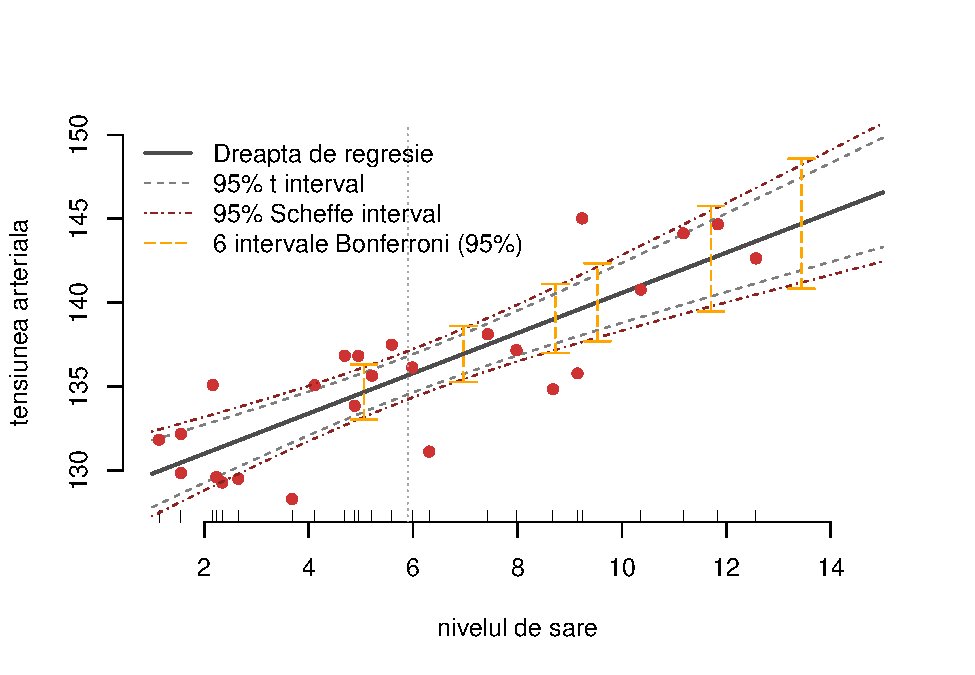
\includegraphics[width=0.9\linewidth]{Lab_7_8_files/figure-latex/unnamed-chunk-24-1}

\}

\textbackslash{}caption\{Nivelul de sare prezis impreuna cu intervalul
de incredere de nivel 95\% pentru raspunsul
mediu\}\label{fig:unnamed-chunk-24} \textbackslash{}end\{figure\}

\subsubsection{Diagnostic}\label{diagnostic}

În această secțiune vom vedea dacă setul nostru de date verifică
ipotezele modelului de regresie liniară.

\begin{itemize}
\tightlist
\item
  \emph{Independența}
\end{itemize}

Ipoteza de independență a variabilei răspuns (prin urmare și a erorilor)
reiese, de cele mai multe ori, din modalitatea în care s-a desfășurat
experimentul.

\begin{itemize}
\tightlist
\item
  \emph{Normalitatea}
\end{itemize}

Pentru a verifica dacă ipoteza de normalitate a erorilor este
satisfăcută vom trasa dreapta lui Henry (sau Q-Q plot-ul):

\begin{Shaded}
\begin{Highlighting}[]
\KeywordTok{library}\NormalTok{(car)}
\end{Highlighting}
\end{Shaded}

\begin{verbatim}
## 
## Attaching package: 'car'
\end{verbatim}

\begin{verbatim}
## The following object is masked from 'package:ellipse':
## 
##     ellipse
\end{verbatim}

\begin{Shaded}
\begin{Highlighting}[]
\KeywordTok{qqPlot}\NormalTok{(saltBP_model, }\DataTypeTok{col =} \StringTok{"brown3"}\NormalTok{, }\DataTypeTok{col.lines =} \StringTok{"grey50"}\NormalTok{, }\DataTypeTok{pch =} \DecValTok{16}\NormalTok{,}
       \DataTypeTok{simulate =} \OtherTok{TRUE}\NormalTok{,}
       \DataTypeTok{xlab =} \StringTok{"Cuantile teoretice"}\NormalTok{,}
       \DataTypeTok{ylab =} \StringTok{"Reziduuri studentizate"}\NormalTok{, }
       \DataTypeTok{main =} \StringTok{"Q-Q plot (Dreapta lui Henry)"}\NormalTok{)}
\end{Highlighting}
\end{Shaded}

\begin{figure}

{\centering 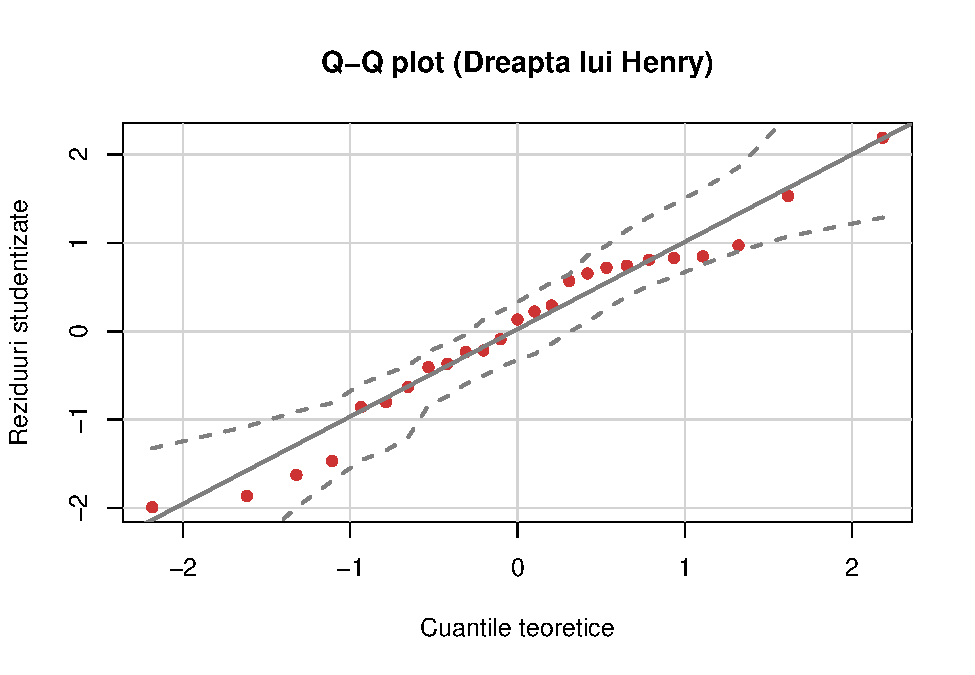
\includegraphics[width=0.9\linewidth]{Lab_7_8_files/figure-latex/unnamed-chunk-25-1} 

}

\caption{Q-Q plot}\label{fig:unnamed-chunk-25}
\end{figure}

Putem folosi și testul \texttt{Shapiro-Wilk}:

\begin{Shaded}
\begin{Highlighting}[]
\KeywordTok{shapiro.test}\NormalTok{(}\KeywordTok{residuals}\NormalTok{(saltBP_model))}
\end{Highlighting}
\end{Shaded}

\begin{verbatim}
## 
##  Shapiro-Wilk normality test
## 
## data:  residuals(saltBP_model)
## W = 0.96871, p-value = 0.6125
\end{verbatim}

\begin{itemize}
\tightlist
\item
  \emph{Homoscedasticitatea}
\end{itemize}

Pentru a verifica proprietatea de homoscedasticitate a erorilor vom
trasa un grafic al reziduurilor versus valorile prezise (fitted), i.e.
\(\hat{\varepsilon}\) vs \(\hat{y}\). Dacă avem homoscedasticitate a
erorilor atunci ar trebui să vedem o variație constantă pe verticală
(\(\hat{\varepsilon}\)).

\begin{Shaded}
\begin{Highlighting}[]
\KeywordTok{plot}\NormalTok{(}\KeywordTok{residuals}\NormalTok{(saltBP_model)~}\KeywordTok{fitted}\NormalTok{(saltBP_model),  }\DataTypeTok{col =} \StringTok{"brown3"}\NormalTok{, }\DataTypeTok{pch =} \DecValTok{16}\NormalTok{, }
     \DataTypeTok{xlab =} \StringTok{"Valori prezise (fitted)"}\NormalTok{,}
     \DataTypeTok{ylab =} \StringTok{"Reziduuri"}\NormalTok{, }
     \DataTypeTok{main =} \StringTok{"Reziduuri vs Fitted"}\NormalTok{,}
     \DataTypeTok{bty =} \StringTok{"n"}\NormalTok{)}

\KeywordTok{abline}\NormalTok{(}\DataTypeTok{h =} \DecValTok{0}\NormalTok{, }\DataTypeTok{col =} \StringTok{"grey30"}\NormalTok{)}
\end{Highlighting}
\end{Shaded}

\begin{figure}

{\centering 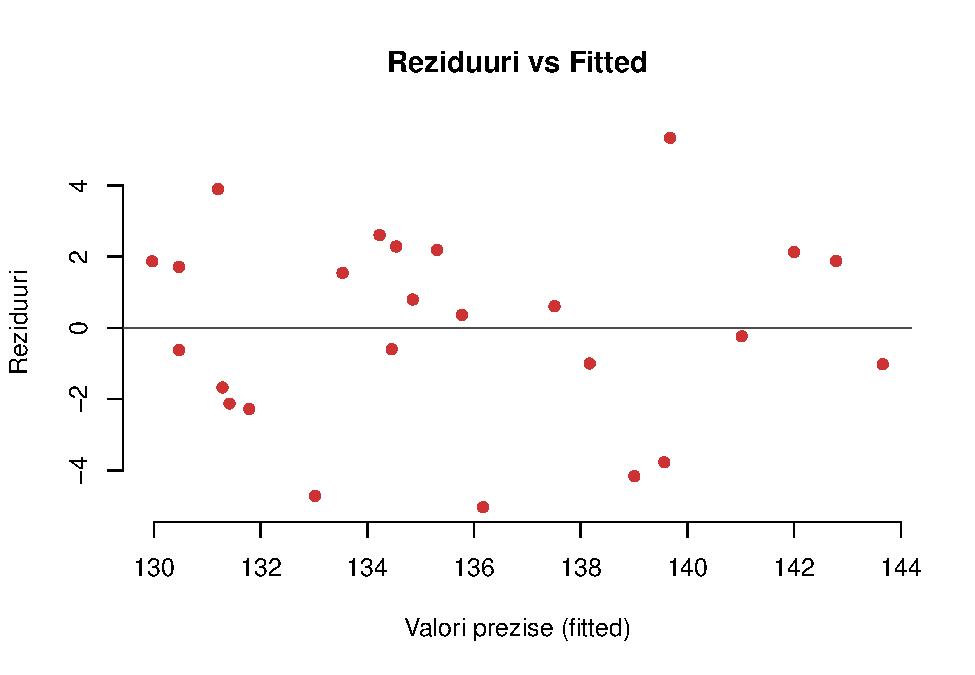
\includegraphics[width=0.9\linewidth]{Lab_7_8_files/figure-latex/unnamed-chunk-28-1} 

}

\caption{Reziduuri vs Valori prezise (Fitted)}\label{fig:unnamed-chunk-28}
\end{figure}

Tot în acest grafic putem observa dacă ipoteza de liniaritate este
verificată (în caz de liniaritate între variabila răspuns și variabila
cauză nu are trebui să vedem o relație sistematică între reziduuri și
valorile prezise - ceea ce se și întâmplă în cazul nostru) ori dacă
există o altă legătură structurală între variabila dependentă (răspuns)
și cea independentă (predictor).


\end{document}
